\section{Acceptance X Efficiency}
\label{sec:AccXEff}

To compute the cross section in a phase space different from our selection criteria, it is necessary to apply the acceptance and efficiency corrections. They are computed in a combined manner as the bin-by-bin correction $A \times \epsilon$ and derived from the signal MC samples.  

The numerator $num$ for the total cross section is determined as the number of selected events in the signal MC with PU weight applied. The numerator $num_i$ for the differential cross section is determined as selected signal MC yields with PU weight applied in $P_T^{\gamma-GEN}$ bins $15-20-25-30-35-45-55-65-75-85-95-120-500$~GeV. 

The denominator $den$ is determined as the number of events that are within the phase space based on their gen-level kinematic values. For the differential cross section, the numbers $den_{i}$ are determined separately for each $P_T^\gamma$ bin.  

The $A \times \epsilon$ correction is determined then as $A \times \epsilon = num/{den}$ for the total cross section and as $(A \times \epsilon)_i = num_i/{den_i}$ for the differential cross section. The $A \times \epsilon$ for the total cross section are
\begin{equation}
(21833 \pm 36)/(177606 \pm 629)=0.1229 \pm 0.0004
\end{equation}
\noindent{for the electron channel, and }
\begin{equation}
(51771 \pm 39)/(179082 \pm 631)=0.2891 \pm 0.0006
\end{equation}
\noindent{for the muon channel. The values for the differential cross section are plotted in Fig.~\ref{fig:covMatricesaccXeff_Wg}.}

\begin{figure}[htb]
  \begin{center}
  \includegraphics[width=0.5\textwidth]{../figs/figs_v11/MUON_WGamma/Constants/C_accXeff_MUON_WGamma.pdf}\includegraphics[width=0.5\textwidth]{../figs/figs_v11/ELECTRON_WGamma/Constants/C_accXeff_ELECTRON_WGamma.pdf}\\
  \label{fig:covMatricesaccXeff_Wg}
  \caption{$A\times\epsilon$ corrections. Left: muon channel, right: electron channel.}
  \end{center}
\end{figure}

%\begin{figure}[htb]
%  \begin{center}
%     \includegraphics[width=0.48\textwidth]{figs_v8/MUON_WGamma/Constants/C_accXeff_MUON_WGamma.pdf} \includegraphics[width=0.48\textwidth]{figs_v8/ELECTRON_WGamma/Constants/C_accXeff_ELECTRON_WGamma.pdf}
%  \caption{Acceptance X Efficiency. Left: MUON channel, right: electron channel.}
%  \label{fig:accXeff_Wg}
% \end{center}
%\end{figure}

The phase space is defined in the following way:
%  Applied at generator-level to compute acceptance and MC-based cross section;\\
%  (tried to follow to the phase space definition of the approved Z$\gamma$ analysis [AN-2013-280] as close as possible)
  \begin{itemize}
  \item $p_T^{\gamma}>15$ GeV;
  \item $\Delta{R}(\gamma,l) > 0.7$;
  \item $|\eta^{\gamma}|<2.5$, $|\eta^{l}|<2.5$;
  \item $p_T^{l}>20$ GeV;
  \item $I^{\gamma}<5$ GeV, where $I_{\gamma}$ is a sum of $P_T$ of all MC generated particles particles $p$ in the event within $\Delta{R(p,\gamma)}<0.3$;
%  \item for Z$\gamma$ Check: M(lep,lep)$>$50 GeV
  \item for differential cross section, $P_T^{\gamma}$ binning: $15-20-25-30-35-45-55-65-75-85-95-120-500$~GeV.
  \end{itemize}

%To determine whether the event within the phase space or not, the following algorithm was used:
%\begin{itemize}
%   \item find a muon/electron which has a W boson as a mother particle
%   \item add 4-momenta of the dressing photons to the 4-momentum of the muon/electron; dressing photons as defined as photons that have $P_T>0.5$ GeV and have $\Delta R(lepton,photon)<0.1$
 %  \item find a final state photon which corresponds to FSR, ISR or TGC; exclude dressing photons from the consideration
 %  \item using 4-momentum of the photon and the adjusted 4-momentum of the lepton, determine whether the event is within the phase space or not
%\end{itemize}

